\documentclass[12pt]{article}

\usepackage[utf8]{inputenc}
\usepackage{setspace}
\usepackage{titlesec}
\newcommand{\sectionbreak}{\clearpage}
\usepackage[utf8]{inputenc}
\usepackage[english]{babel}
\usepackage{fancyhdr}
\pagestyle{fancy}
\onehalfspacing
\usepackage{graphicx}
\usepackage{fontspec}
\renewcommand{\listfigurename}{ILLUSTRATIONS}

\setmainfont[Path=/usr/share/fonts/TTF/,
BoldItalicFont=timesbi.ttf,
BoldFont      =timesbd.ttf,
ItalicFont    =timesi.ttf]{times.ttf}

\renewcommand*\contentsname{TABLE OF CONTENTS}
\fancyhead[L]{\includegraphics[width=1.5cm]{/home/muiz_bspwm/Pictures/assets/uow.png}}
\fancyhead[R]{\includegraphics[width=1.5cm]{/home/muiz_bspwm/Pictures/assets/iit.png}}
\renewcommand{\headrulewidth}{0.1pt}
\thispagestyle{plain}
\begin{document}
\begin{titlepage}
\begin{center}
    {\Large\bfseries INFORMATICS INSTITUTE OF TECHNOLOGY \\ in collaboration with \\
    the University of Westminster, UK\\}
\vspace{1cm}
{\Large \bfseries BEng (Hons) DEGREE PROGRAMME in \\ Software Engineering\\}
\vspace{2.5cm}
{\Large\bfseries REPORT ON INDUSTRIAL PLACEMENT \\ of \\ A. Muiz Uvais\\}
\vspace{2cm}
{\Large in relation to the work carried out at \\ iTelaSoft \\ 69 Old Kottawa Rd, Nugegoda 10250 \\ 2020\\}

\end{center}

\end{titlepage}

\section*{Acknowledgement}
I would like to sincerely thank and acknowledge iTelaSoft,
and it's management for giving me the opportunity for giving 
me the opportunity for me to do my Industrial Placement.
\newline
\newline
I would also like to thank the my supervisors
Manoj, and Deepan for guiding me through the industrial placement. \newline \newline 
Last but not least
I also would like to thank my colleagues at team EFFI who helped me out when I got stuck or was new to
certain areas.
\newpage

\tableofcontents

\pagenumbering{roman} % Start roman numbering
\listoffigures

\section*{ABBREVIATIONS}
{\large IIT -- (The) Informatics Institute of Technology\\}
\newline
{\large SE -- Software Engineering\\}
\newline
{\large UoW -- University of Westminster\\}
\newline
{\large IT -- Information Technology\\}
\newline
{\large IP -- Industrial Placement\\}
\newpage


\pagenumbering{arabic} % Switch to normal numbers
\section{Introduction}
An Industrial Placement is an experience where the intention is to prepare the student for their
future employment, therefore the industrial placement is an integral part of the process of 
entering the SE industry. As an SE student I feel extremely fortunate that IIT in collaboration with
the UoW has given this path for students enrolled in this course.\\
\newline
While working at iTelaSoft I was able to gain experience working in a lot of areas. These areas included 
front-end as well as a bit of work in the back-end. Although I did more work in the front-end, I have
also gained an insight into back-end. I feel that I have benefited greatly from my exposure to those 
technologies. However, I have also gained exposure to soft skills which has been equally beneficial
to me. Working for a company like iTelaSoft I have been able to learn to deal with tough situations
that would usually come up in the industry. Therefore I can safely conclude that the IP will play
an foundational role in my career.\\
\newline
At work I received a lot of support from my team members. I worked in the web development field which
is the main scope of the company, most of my co-workers were well experienced, and extremely helpful
to me.\\
\newline
I started my placement on the 02st of July 2019, and completed it on the 01st of July 2020. While 
there were obstacles I faced it was an important experience that I will always remember.


\section{Company Profile}
iTelaSoft is an Australian-owned company which provides IT services, and Software Product Development,
which is located at 69 Old Kottawa Rd, Nugegoda 10250. It 
specializes in strategy consultation, development, and management of products.\\
\newline
In 2009 a group of IT veterans founded the company which is known
today as iTelaSoft. The founders who specialized in
enterprise technology, and product development set out with a vision of enabling
small to medium scale organization who seek the latest technology solutions. The mission statement of
iTelaSoft is ``Empower our customers to prosper through sustained innovation''.\\
\newline
iTelaSoft is headquartered in Australia while having development hubs in South Asia, namely Sri Lanka, and India.
Over the span of the decade iTelaSoft has and continues to provide 
solutions to a diverse range of markets essentially setting itself
up as a leading development firm. iTelaSoft has provided services for clients who belong to various markets
such as Education, Retail, Telco, Fintech, et al. which is evidence of the company's versatility.
While at iTelaSoft I worked as a Software Engineering Trainee.\\
\newline
Considering the figure below, it is safe to assume that iTelaSoft follows a hierarchical, and centralized organization 
structure.\\
\newpage

\begin{figure}
  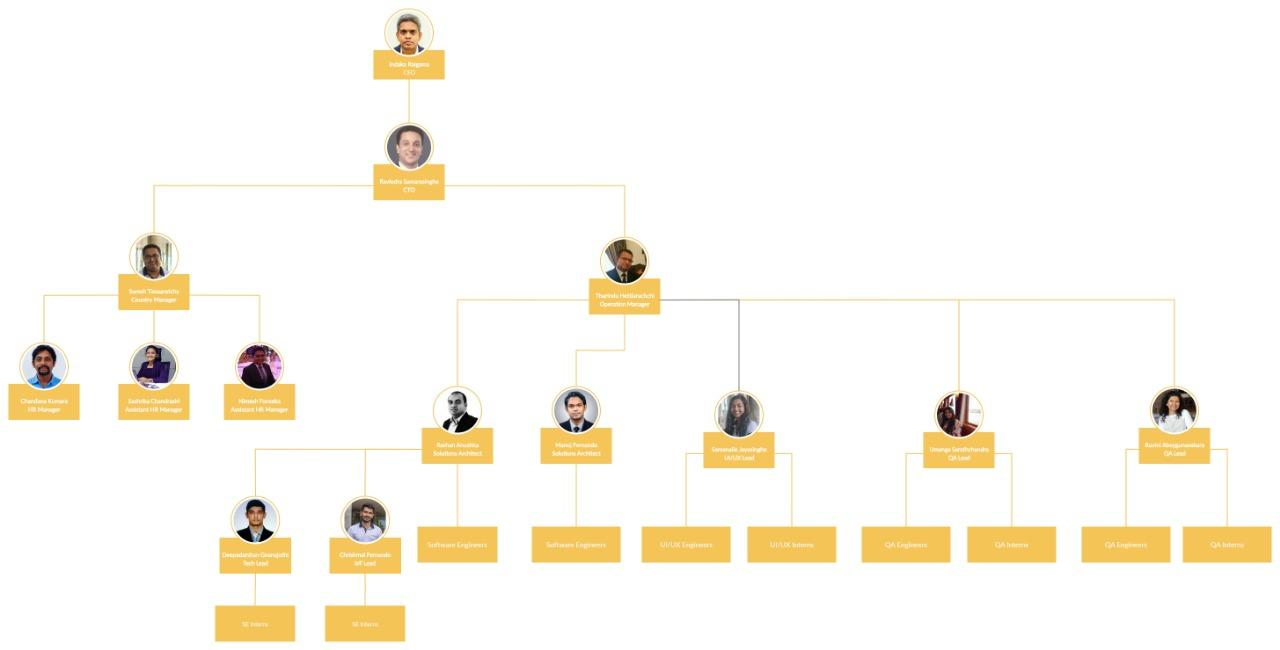
\includegraphics[width=\linewidth]{its_org_structure.jpg}
  \caption{iTelaSoft Organization Structure}
  \label{fig:org_structure}
\end{figure}
\newpage

\section{Work carried out}
During my placement year I was given the opportunity to work in two different projects.
\begin{enumerate}
    \item TimeTapp
    \item Effi
\end{enumerate}
\subsection{TimeTapp}
TimeTapp is an application which records employees' work hours as well as their break hours. Although timetapp is
a mobile application, it has a dashboard for the administrator as well.\\
\newline
The resources used for the timetapp dashboard were nuxt js for the front-end and dotnet entity framework for the API, the
mobile application was developed using flutter.
For the front-end section I was allocated tasks such as creating pages, and adding components to the pages. 
In addition to the front-end I was also allocated minor tasks in the back-end such as creating new entities, and 
adding requests to the controller. This was the part where I had the most problems as I initially did not have 
a deep understanding of the entity framework, however after careful reading of the documentation, and the advice of 
my peers I was able to get a better understanding. Overall I would say that this task gave a lot of insight.\\



 \begin{figure}[ht]
  
\includegraphics[width=3cm]{timetapp.png}
  \caption{TimeTapp Logo}
  \label{fig:timetapp}
\end{figure}

\subsection{Effi}
EFFI, the smartest mortgage broker platform ever built. Is a site where brokers can connect with clients, so they 
can deliver broker services to their clients. \\
\newline
The resources used for EFFI were nuxt js for the front-end, and dotnet entity-framework core for the backend, the 
mobile application was developed using flutter.\\
\newline
I was assigned the task of developing components and pages of the domains. I faced issues initially with state management
in nuxt but later I was able figure how the system worked.\\
\newline
I would say that EFFI was the longest project I worked with. It was a project where we had to start from scratch
and it was very interesting to work with, I gained some insight about how the Australian mortgage brokering system works
through this.

 \begin{figure}[ht]
  
\includegraphics[width=3cm]{effi.png}
  \caption{Effi Logo}
  \label{fig:effi}
\end{figure}

\section{Observations}
Between starting and finishing my IP, I have gained a paradigm shift in many ways. I have been able to work with teams
and synergize with members of those teams very effectively. I have had the privilege of working with people who 
have had a lot of experience in the industry, which exposed me to the best techniques both in development as well
as the professional setting.\\
\newline
iTelaSoft treats it's employees exceptionally well. The environment at iTelaSoft among co-workers
is extremely friendly. iTelaSoft has a really great culture where everyone is cooperative and is friendly.\\
\newline
iTelaSoft also helped me in my professional career as well, I was able to learn new, yet popular technologies
such as nuxt js which I have become increasingly familiar with. I also gained knowledge in dotnet entity framework.
I was also able to grasp concepts such as CI/CD (continuous integration/ continuous integration).\\
\newline
iTelaSoft has also been able to provide events such as iTelaNight, Movie night, et al. These events were really
enjoyable and a great way for staff to meet and interact with each other outside of a work environment. When it 
is someone's birthday we usually have a celebration, as well as a second celebration at the end of the month for 
everyone who had their birthdays on that month. Employees who work late are compensated with free transport, and 
were offered free meals. Overall it was a positive experience to work at iTelaSoft, and I as someone who worked 
with web development I would recommend anyone who wants to join.\\
\newpage


%\begin{appendices}
%\end{appendices}
\end{document}
